\section{Appendix of the Analysis of 4 Lepton Channel }
\label{sec:AppAnaFourL}

\subsection{Analysis strategy}
\label{subsec:ana}

This analysis relies on the use of a multivariate discriminant designed to select candidate events consistent with non-resonant $HH$ production. To construct such a discriminant, a signal region is defined with some event selection criteria. Section \ref{subsubsec:pre-selection} describes these signal region selection criteria. Section \ref{subsubsec:mva} describes the architecture and the training of the Boosted Decision Tree (BDT) classifier from which the discriminant is constructed. Section \ref{subsubsec:bkg} describes the final background estimation procedure.

\subsubsection{Event selection}
\label{subsubsec:pre-selection}

To define the signal criteria, the analysis has some further requirements on each event. These events are triggered by any of the standard single electron and single muon, or di-leptons. Then trigger matching is applied to data and MC, requiring any of the selected leptons to be close to the corresponding trigger lepton within $\Delta{R}<0.1$.

In $4l+b\bar{b}$ channel, signal event are selected with exactly four leptons. The four leptons are sorted by $p_{T}$ number. Either of the third lepton and the forth lepton, with the third and forth highest $p_{T}$, is required to pass the $PflowLoose$ isolation working point. This loose selection can give a acceptable background rejection and good signal efficiency.

A angular separation of $\Delta{R}(l_{i},l_{j})=\sqrt{(\eta_{i}-\eta_{j})^{2}+(\phi_{i}-\phi_{j})^{2}}<0.1$ is required between any of lepton pairs.

In each quadruplet, the $p_{T}$ thresholds for the three leading leptons are 20,15 and 10 GeV.

The invariant mass of the $OSSF$ lepton pairs in each quadruplet is calculated. The lepton pair with invariant mass closest to the nominal $Z$ boson mass is selected as the leading lepton pair. The two remaining leptons are also required to be $OSSF$ and form the sub-leading lepton pair.

All the $OSSF$ lepton pairs are required to have invariant mass large than 5 GeV to veto the $J/\Psi$ decay.

Events are selected with at least two jets. The $DL1r$ algorithm is used to identify jets containing $b$-hadrons ($b$ jets). Events containing at least one $b$ jets are selected by requiring the number of jets passing a $DL1r$ working point, which gives a $b$-tagging efficiency of 77\%, no less than one.

Finally the invariant mass of the four leptons must satisfy 107 GeV$<M_{\rm 4l}<$ 133 GeV to select a on-shell Higgs decay. A comprehensive summary of all the cuts and requirements used in the event selection is shown in Table \ref{Tab.pre-selection}.

\begin{table}[H]
\begin{center}
\caption{The event selection used to define the signal criteria.}
\label{Tab.pre-selection}
\begin{tabular}{cc}
	\toprule
	\toprule	
	\multicolumn{2}{c}{\textbf{Event Selection}}\\
	\midrule
	\textbf{Trigger Matching}&Medium\\
	\midrule
	\textbf{Isolation}&\makecell[c]{Either of the third lepton and the forth lepton\\ passes the $PflowLoose$ isolation working point}\\
	\midrule
	\textbf{Separation}&$\Delta{R}(l_{i},l_{j})=\sqrt{(\eta_{i}-\eta_{j})^{2}+(\phi_{i}-\phi_{j})^{2}}<0.1$\\
	\midrule
	\textbf{Kinematics}&$p_{T}$ > 20, 15, 10 GeV for the three leading leptons\\
	\midrule
	\textbf{Pair Selection}&Two $OSSF$ lepton pairs\\
	\midrule
	\textbf{$J/\Psi$ veto}&All $OSSF$ lepton pairs have mass large than 5 GeV\\
	\midrule
	\textbf{Jets Number}&$N_{\rm jets}\ge{2}$\\
	\midrule
	\textbf{b Jets Number}&$N_{\rm b jets}\ge{1}$\\
	\midrule
	\textbf{Quadruplet Mass}&107 GeV $<M_{\rm 4l}<$ 133 GeV\\
	\bottomrule
	\bottomrule
\end{tabular}
\end{center}
\end{table}

\subsubsection{Multi-variable analysis}
\label{subsubsec:mva}

To enhance sensitivity to the signal process and to maximize rejection of the expected SM backgrounds, some observables from the selected events are checked and used for building a multivariate discriminant. The input variables are list in Table \ref{Tab.bdt inputs}. Distributions of these inputs are shown in Figure \ref{Fig.inputs}. This discriminant uses the outputs of a BDT classifier trained with the Toolkit for Multivariate Analysis (TMVA) which provides a ROOT-integrated environment for the processing.

\begin{table}[H]
\begin{center}
\caption{Variables used as inputs to the BDT classifier.}
\label{Tab.bdt inputs}
\begin{tabular}{cc}
	\toprule
	\toprule	
	Variables&Description\\
	\midrule
	$lep\_p_{T}\_*,lep\_\Phi\_*,$&$p_{T},\Phi$ of all the four leptons\\
	\midrule
	$jet\_p_{T}\_*,jet\_E\_*,jet\_\Phi\_*,$&$p_{T},E,\Phi$ of the two leading jets\\
	\midrule
	$M_{12},M_{34},M_{4l},M_{jj}$&\makecell[c]{Invariant mass of the leading lepton pair, \\sub-leading lepton pair, quadruplet and leading jets pair}\\
	\midrule
	$p_{T,4l},p_{T,jj}$&$p_{T}$ of the quadruplet and the leading jets pair\\
	\midrule
	MET&Missing transverse energy\\
	\midrule
	$cos\theta_{12},cos\theta_{34}$&\makecell[c]{Cosine of the angle between two leptons \\in the leading pair and sub-leading pair}\\
	\midrule
	$cos\theta_{pairs}$&Cosine of the angle between two lepton pairs\\
	\midrule
	$\Delta\Phi_{MET\&jets}$&$\Delta\Phi$ of the MET and leading jets\\
	\midrule
	$N_{jets},N_{bjets}$&The number of jets and b jets\\
	\bottomrule
	\bottomrule
\end{tabular}
\end{center}
\end{table}

\begin{figure}[H]
	\caption{Distributions of inputs for BDT training.}
	\label{Fig.inputs}
	\centering
	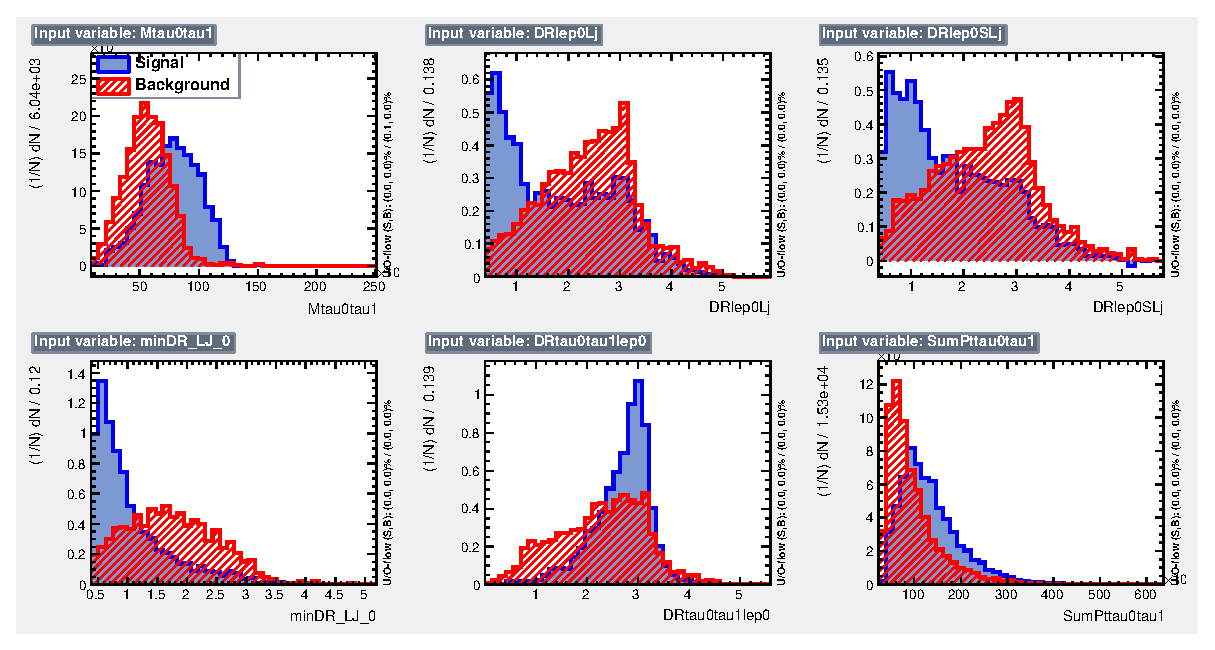
\includegraphics[width=0.4\textwidth]{figures/variables_id_c1.eps}
	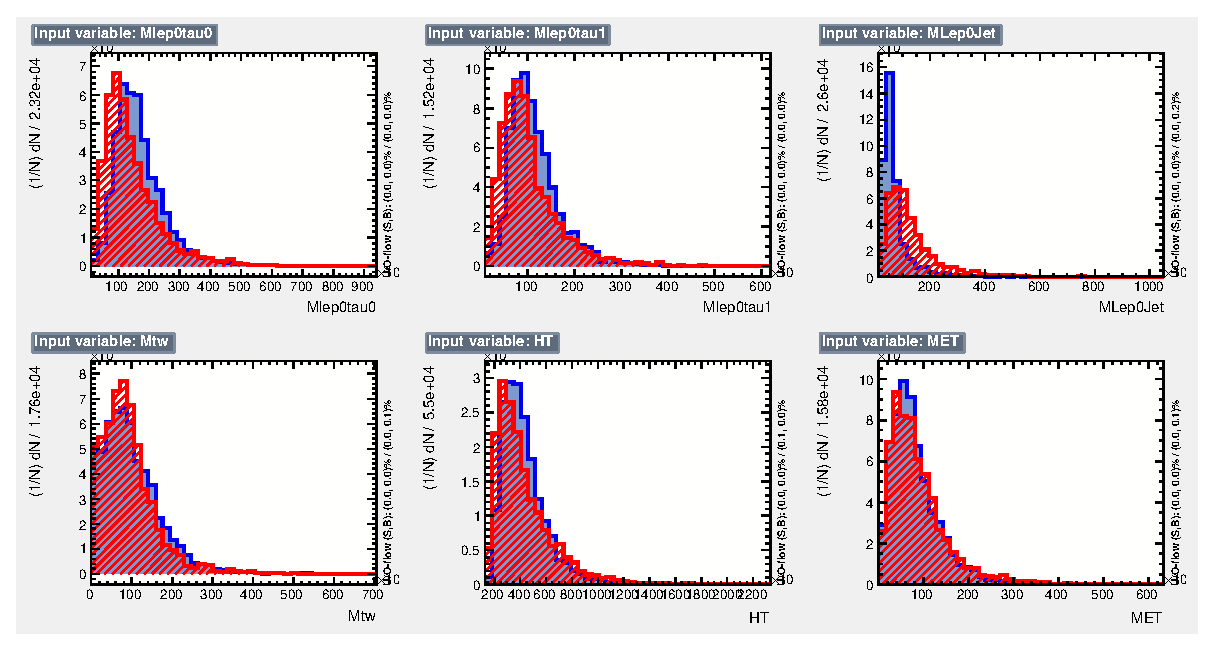
\includegraphics[width=0.4\textwidth]{figures/variables_id_c2.eps}
	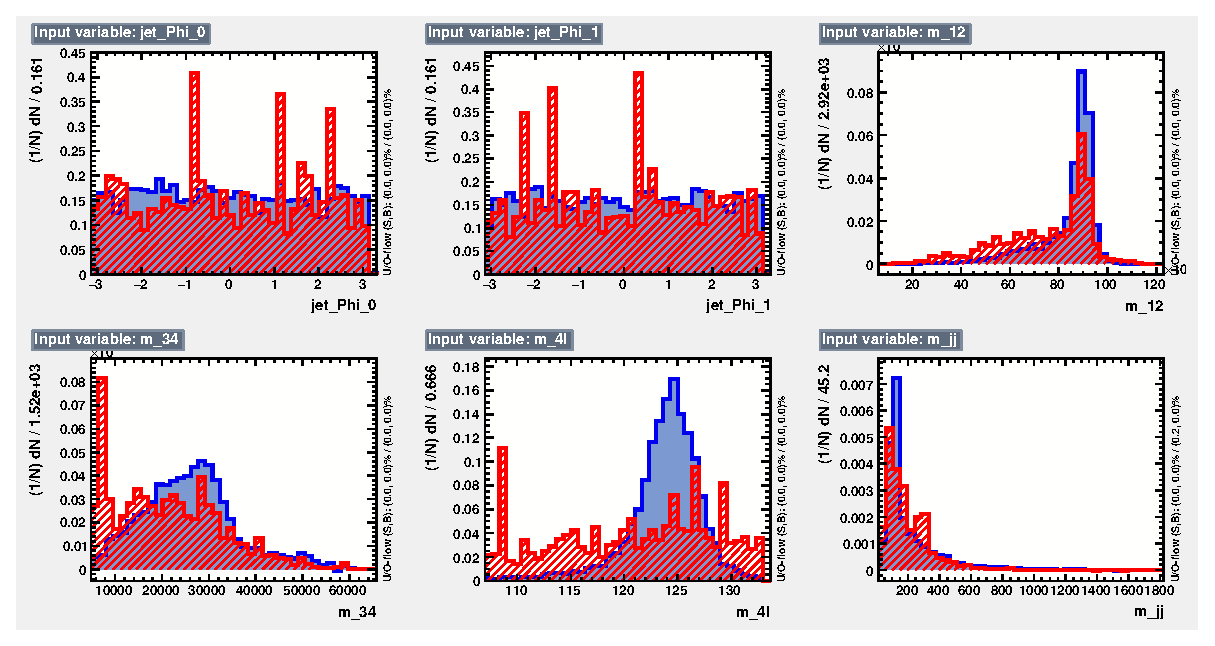
\includegraphics[width=0.4\textwidth]{figures/variables_id_c3.eps}
	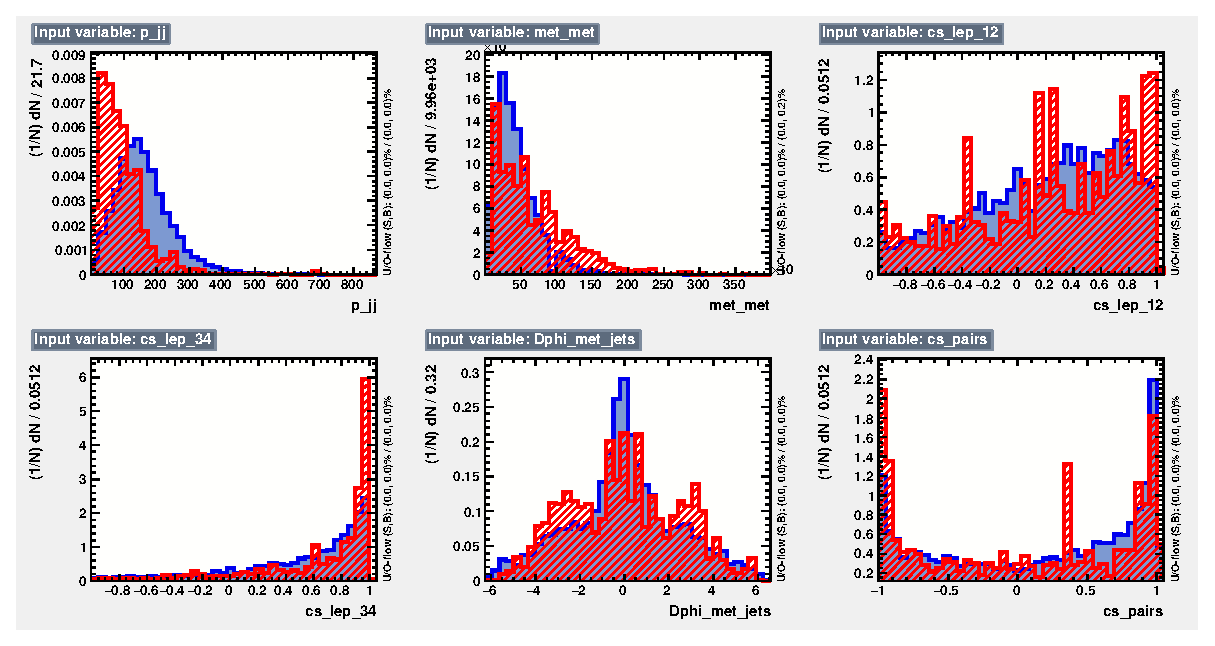
\includegraphics[width=0.4\textwidth]{figures/variables_id_c4.eps}
	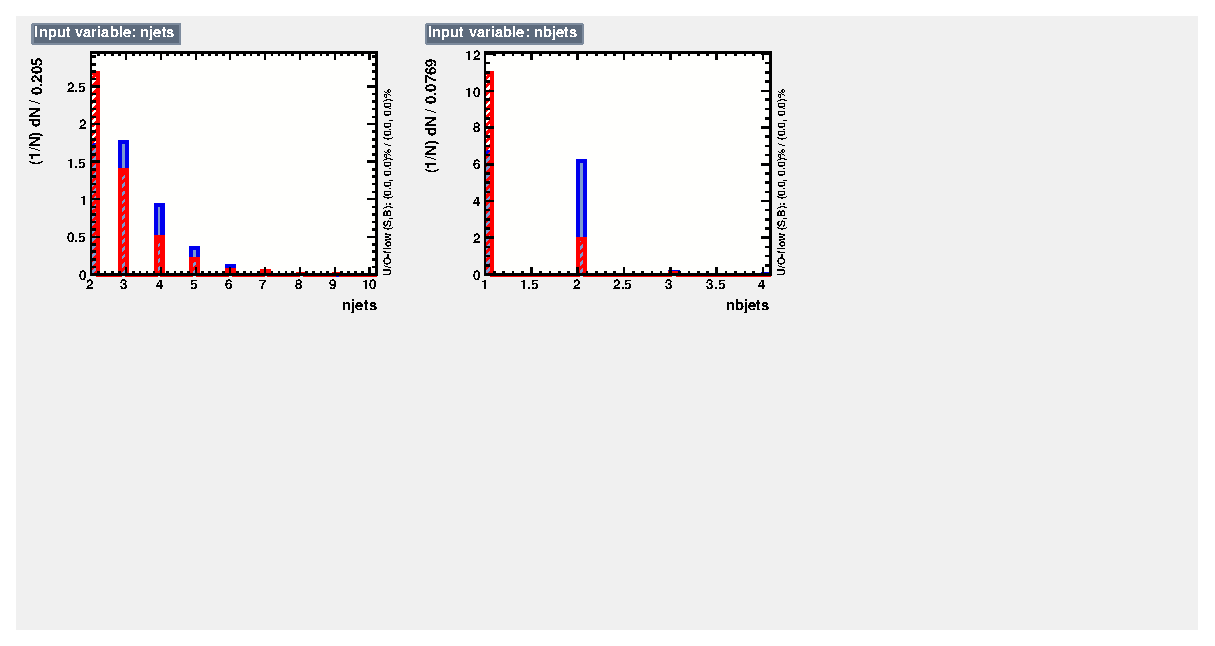
\includegraphics[width=0.4\textwidth]{figures/variables_id_c5.eps}
\end{figure}

Events used for training is composed of randomly 90\% of the total events from the signal  and full backgrounds which pass the event selection. The rest of events are used for testing. The overtraining results is shown in Figure \ref{Fig.overtraining}. More details about the setup of the training can be found in Appendix \ref{app.bdt}

\begin{figure}[H]
	\caption{BDT overtraining results.}
	\label{Fig.overtraining}
	\centering
	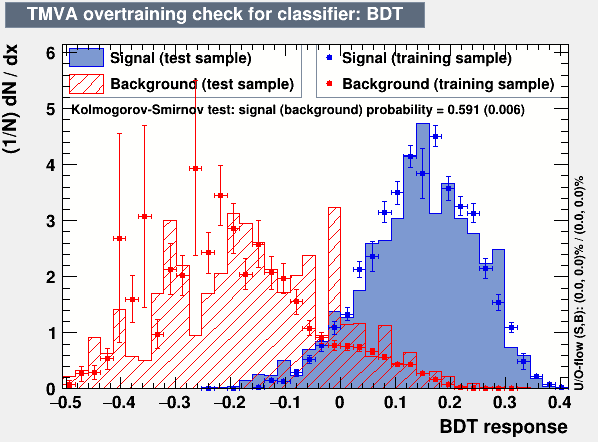
\includegraphics[width=0.6\textwidth]{figures/overtrain_BDT.png}
\end{figure}

The classifier obtained from this training is applied on total signal and background samples and produces the outputs, i.e. BDT scores, of which the values vary between -0.6 to 0.4. The distribution of BDT score in SR is shown in Figure \ref{Fig.SR pre-fit}. 

\begin{figure}[H]
	\caption{BDT score distribution in SR. Dashed line represents signal normalized to total background}
	\label{Fig.SR pre-fit}
	\centering
	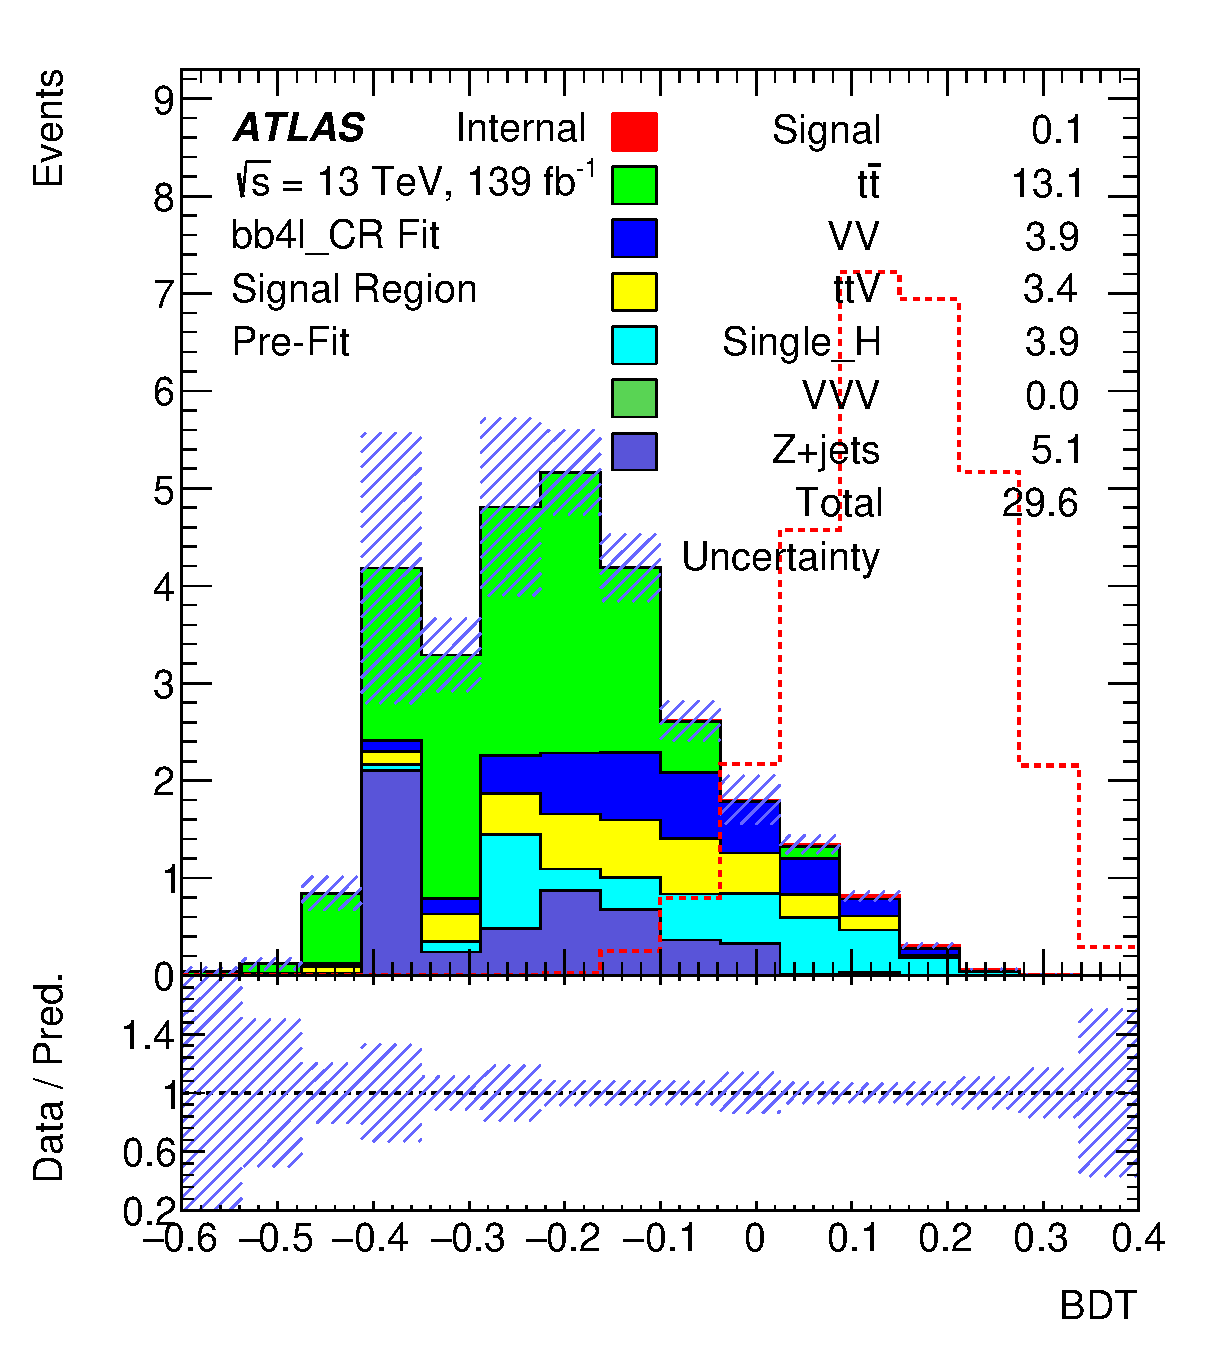
\includegraphics[width=0.6\textwidth]{figures/Plots/SR.eps}
\end{figure}

\subsubsection{Background estimation}
\label{subsubsec:bkg}

As mentioned in Section \ref{sec:sample}, the dominant backgrounds in $4l+b\bar{b}$ channel include $t\bar{t}$, $t\bar{t}Z$, diboson, single Higgs and $Z$+jets processes. Since the signal selection uses some relatively loose cuts to improve the signal efficiency, processes with large cross section, like $t\bar{t}$, diboson and $Z$+jets, can have more events surviving from the selection and have the major contribution to the total backgrounds. Some other processes with exactly the same topology as the signal, like $t\bar{t}Z$ and Higgs production, also have some important contribution. To estimate these dominant backgrounds, several dedicated control regions (CRs) are defined to derive normalization corrections for the MC results in signal region (SR): $t\bar{t}$ CR for $t\bar{t}$, $t\bar{t}Z$ CR for $t\bar{t}Z$, $VV$+Higgs CR for the combination of diboson with single Higgs, and $Z$+jets CR for $Z$+jets. These normalization corrections have a uniform prior and are checked in a validation region (VR).

\paragraph{CR definitions}

In principle, the definitions of CRs should be as similar as possible with SR and satisfy that each CR is orthogonal to SR. This ensures that the normalization correction determined in the fit for the background results in an accurate estimate of the dominant backgrounds process in the signal regions. In this case, the following description will only mention about the differences between CRs with SR. The other definitions of CRs are kept the same with the event selection in SR which are mentioned in Section \ref{subsubsec:pre-selection}.

For the $t\bar{t}$ CR, the sub-leading lepton pair is required not to be $OSSF$ ($anti$-$OSSF$), which builds a phase space orthogonal to SR. The leading lepton pair should satisfy $M_{\rm leading\ pair}<$ 75 GeV or $M_{\rm leading\ pair}>$ 100 GeV to veto the $Z$ decay.

For the $t\bar{t}Z$ CR, the sub-leading lepton pair is required to be $anti$-$OSSF$. All the four leptons must pass the isolation with $PflowLoose$ working point to suppress $t\bar{t}$ process. The leading lepton pair should satisfy 85 GeV $<M_{\rm leading pair}<$ 100 GeV to suppress the processes without $Z$ decay. The requirement on the invariant mass of the quadruplet is removed to enhance $t\bar{t}Z$ process.

For the $VV$+Higgs CR, events are required to containing no $b$ jets by zero jets passing the $DL1r$ working point, which build a phase space orthogonal to SR. Also all the four leptons are required to pass the isolation.

For the $Z+$jets CR, the sub-leading pair is required to be $anti$-$OSSF$. The leading lepton pair should satisfy 85 GeV $<M_{\rm leading pair}<$ 100 GeV to suppress the processes without $Z$ decay. The missing transverse energy (MET) should satisfy $MET<$ 80 GeV to suppress $t\bar{t}$ process. The requirement on the number of $b$ jets is removed to enhanced $Z$+jets process.

Table \ref{Tab.CRs summary} gives a summary about all of the differences of these CRs compared with SR. The BDT classifier mentioned in Section \ref{subsubsec:mva} is applied to the data and MC results from all above CRs to obtain the BDT score distributions in each CR. The results are shown on Figure \ref{Fig.CRs pre-fit}.

\begin{table}[H]
\begin{center}
\caption{Control regions definition, only the differences with signal region listed.}
\label{Tab.CRs summary}
	\begin{tabular}{c|c}
		\toprule
		\toprule
		\multirow{2}{*}{$t\bar{t}$ CR}&$\ast$Sub-leading pair $anti$-$OSSF$\\
		&$\ast{M_{\rm leading\ pair}<75}$ GeV || $M_{\rm leading\ pair}>100$ GeV\\
		\midrule
		\multirow{4}{*}{$t\bar{t}V$ CR}&$\ast$Sub-leading pair $anti$-$OSSF$\\
		&$\ast$All four leptons pass the isolation\\
		&$\ast$85 GeV $<M_{\rm leading\ pair}<$ 100 GeV\\
		&$\ast$No requirement on $M_{\rm 4l}$\\
		\midrule
		\multirow{2}{*}{$VV$+Higgs CR}&$\ast{N_{\rm bjets}=0}$\\
		&$\ast$All four leptons pass the isolation\\
		\midrule
		\multirow{4}{*}{$Z$+jets CR}&$\ast$Sub-leading pair $anti$-$OSSF$\\
		&$\ast$85 GeV $<M_{\rm leading\ pair}<$ 100 GeV\\
		&$\ast{MET<80}$ GeV\\
		&$\ast$No requirement on $N_{\rm bjets}$\\
		\bottomrule
		\bottomrule
	\end{tabular}
\end{center}
\end{table}

\begin{figure}[H]
	\caption{Pre-fit results in each CR, the upper left one is $t\bar{t}$ CR, the upper right one is $t\bar{t}$V CR, the bottom left one is $VV$+Higgs CR, the bottom left one is $Z$+jets CR.}
	\label{Fig.CRs pre-fit}
	\centering
	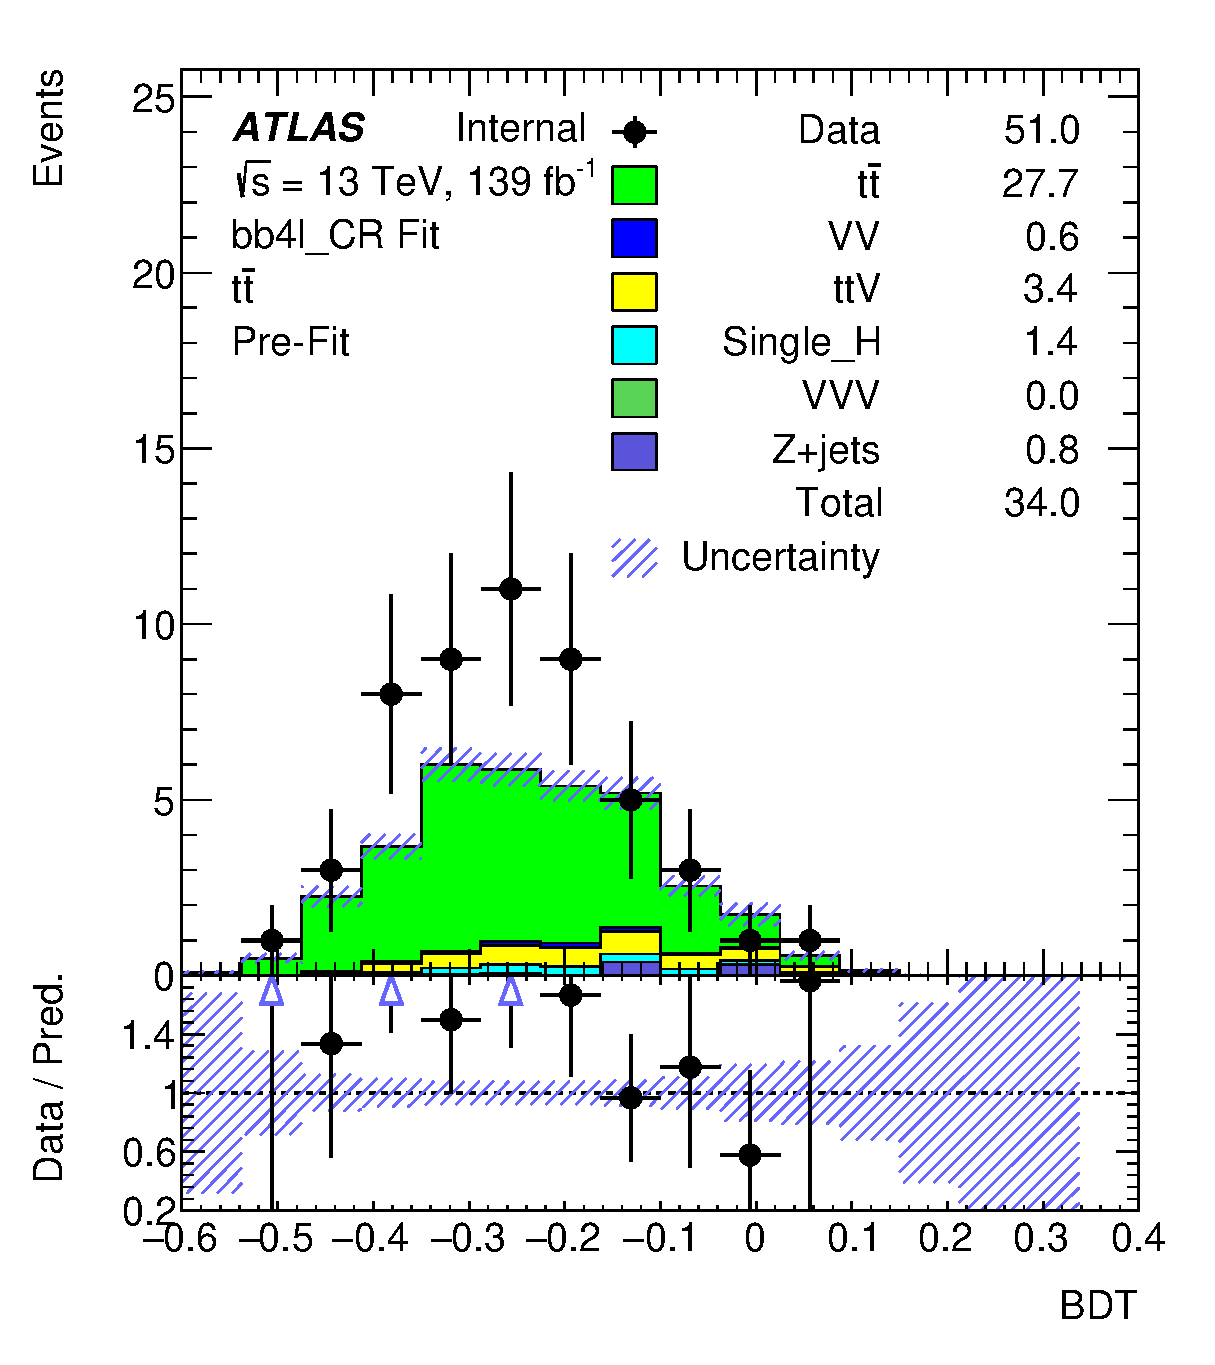
\includegraphics[width=0.4\textwidth]{figures/Plots/tt_CR.eps}
	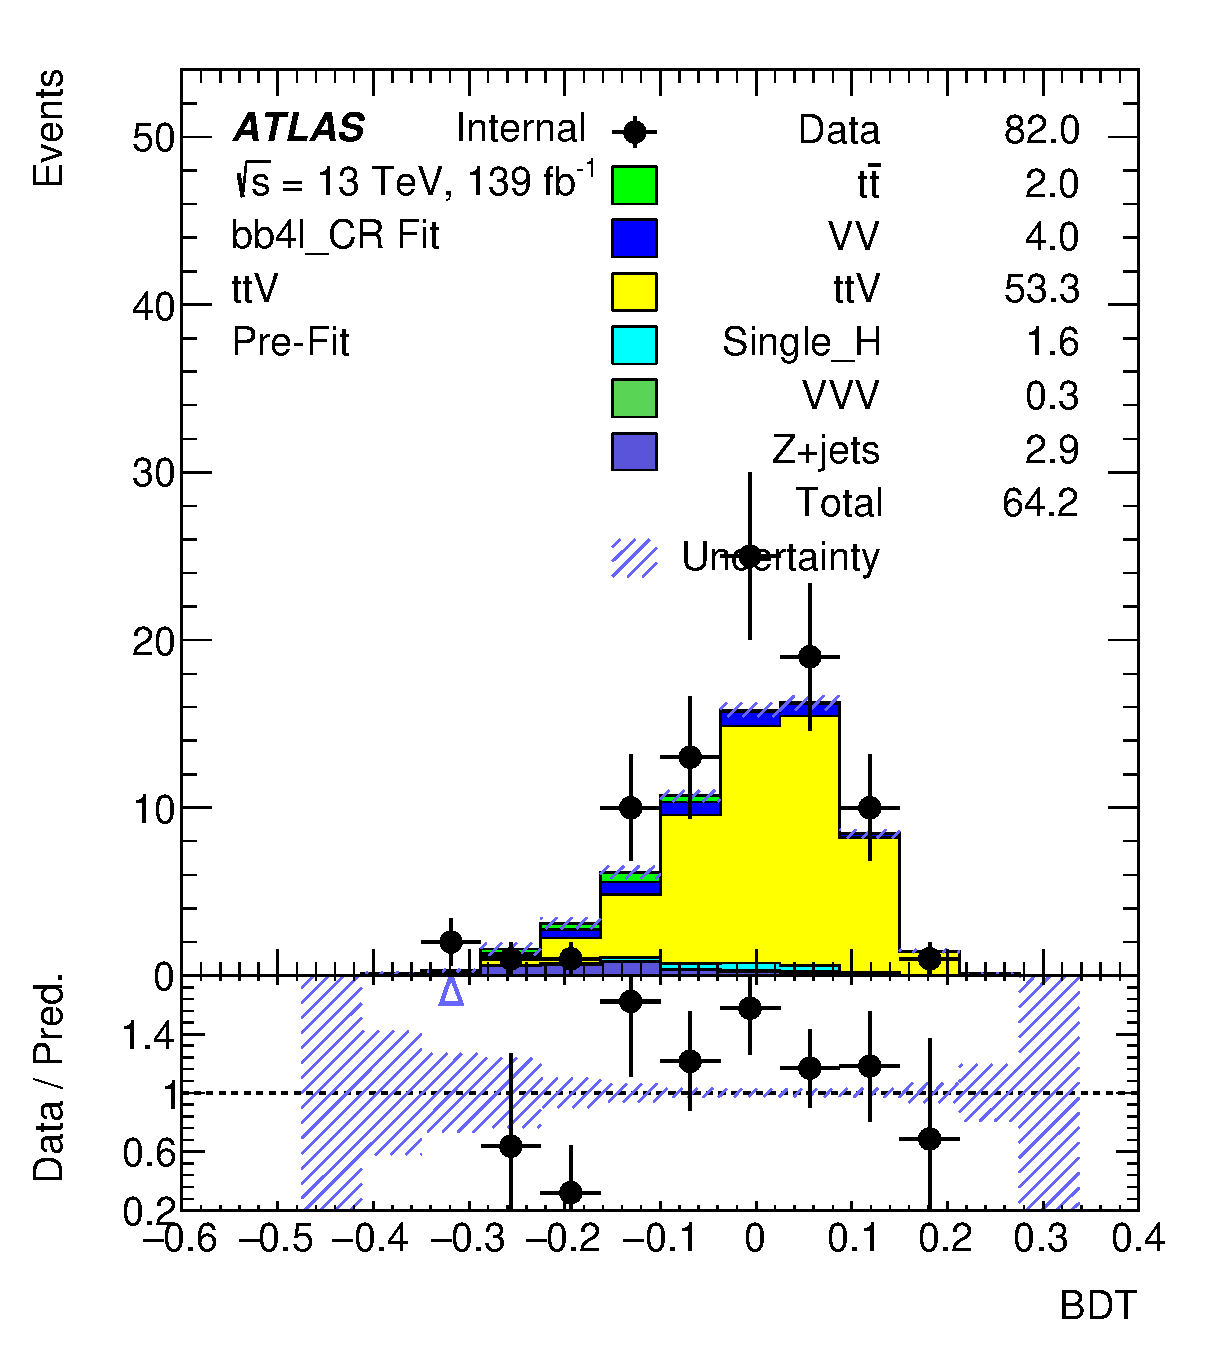
\includegraphics[width=0.4\textwidth]{figures/Plots/ttV_CR.eps}
	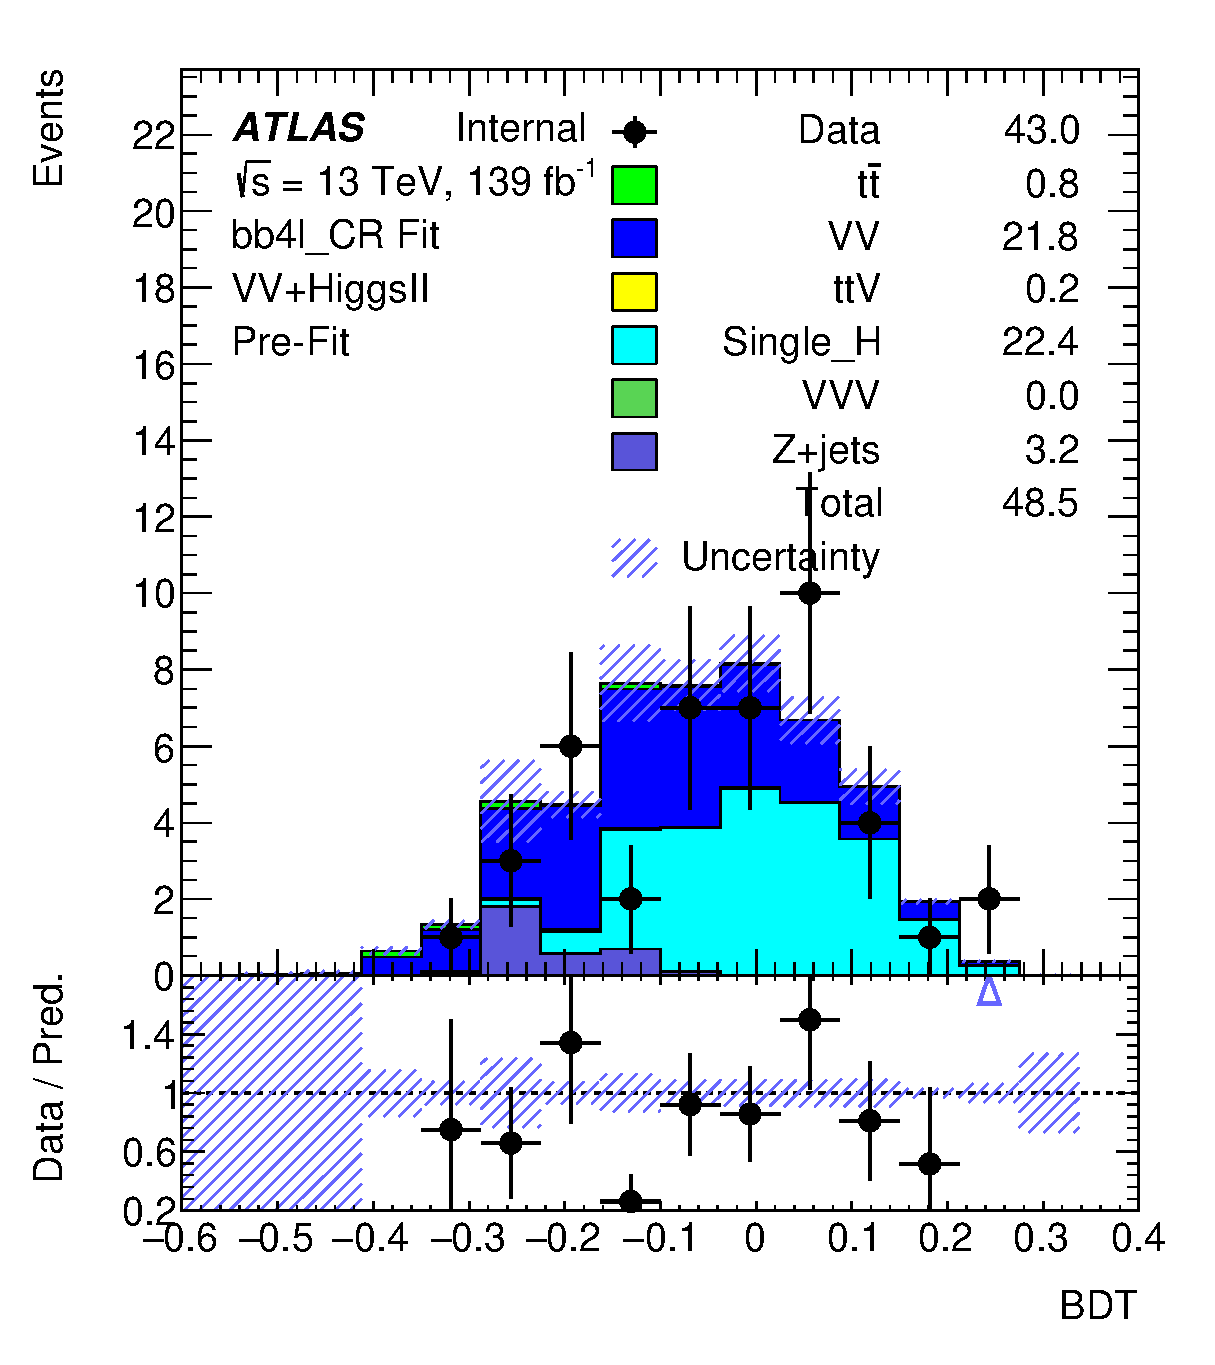
\includegraphics[width=0.4\textwidth]{figures/Plots/VVHiggsII_CR.eps}
	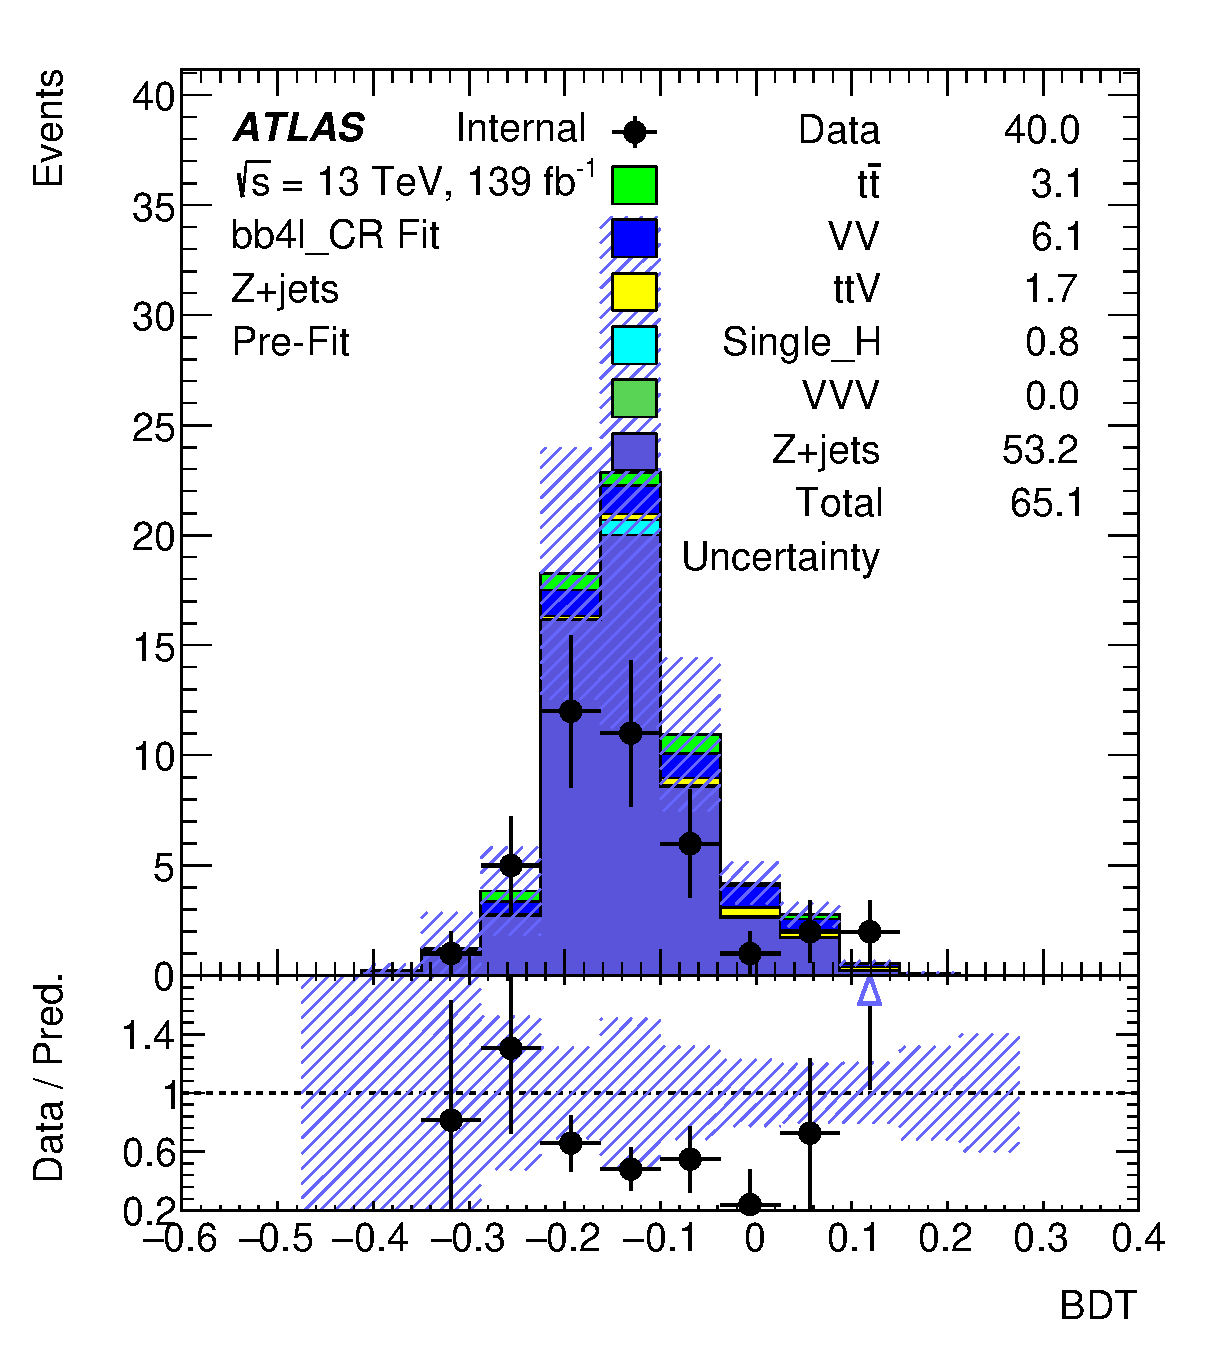
\includegraphics[width=0.4\textwidth]{figures/Plots/Zjets_CR.eps}
\end{figure}

\paragraph{Fitting and validation}

The normalization corrections on MC results are derived from the background-only fits to data in the CRs. Distributions of BDT score are used to do this fitting as they contain the combined information from the observables listed in table, which can avoid strong correlation on some specific observables between CRs with SR or VR to ensure that the corrections can be extrapolated.

Table \ref{Tab.yields} compares the observed and predicted event yields, where the background event yields obtained after background-only fits in the corresponding control regions are also shown. The post-fit normalization correction factors for the dominant background processes, respectively $\mu_{t\bar{t}}=1.51\pm0.23,\mu_{t\bar{t}Z}=1.35\pm0.17,\mu_{VV}=0.77\pm0.39,\mu_{\rm Higgs}=1.12\pm0.37$, and $\mu_{Z+{\rm jets}}=0.5\pm0.18$, are also shown in Table \ref{Tab.yields}.

\begin{table}[H]
\begin{center}
\caption{Analysis region and background estimation summary, only statistical uncertainties included.}
\label{Tab.yields}
	\begin{tabular}{cccccc}
		\toprule
		\toprule
		\multicolumn{6}{c}{\textbf{Event Yields}}\\
		\midrule
		&$t\bar{t}$ CR&$t\bar{t}Z$ CR&$VV$+Higgs CR&$Z$+jets CR&VR\\
		\midrule
		Data	&51$\pm$7&82$\pm$9&43$\pm$7&40$\pm$6&303$\pm$17\\
		\midrule
		Total Bkg.&33.17$\pm$1.43&64.16$\pm$0.88&48.47$\pm$1.92&65.05$\pm$13.37&251.42$\pm$2.57\\
		\midrule
		$t\bar{t}$&31.53$\pm$1.18&2.23$\pm$0.31&0.96$\pm$0.21&3.54$\pm$0.40&61.15$\pm$1.56\\
		$t\bar{t}Z$&3.71$\pm$0.16&59.67$\pm$0.60&0.27$\pm$0.04&1.94$\pm$0.11&92.15$\pm$0.73\\
		$VV$	&0.60$\pm$0.06&4.05$\pm$0.16&21.77$\pm$0.28&6.13$\pm$0.23&79.05$\pm$0.51\\
		Higgs	&1.44$\pm$0.03&1.60$\pm$0.03&22.41$\pm$1.51&0.84$\pm$0.62&9.43$\pm$0.71\\
		$Z$+jets&0.05$\pm$0.79&2.85$\pm$0.54&3.09$\pm$1.14&51.89$\pm$13.33&9.15$\pm$1.69\\
		\midrule
		\midrule
		\multicolumn{6}{c}{\textbf{Post-fit Normalization}}\\
		\midrule
		\multicolumn{6}{c}{$\mu_{t\bar{t}}=1.51\pm0.23\mid\mu_{t\bar{t}Z}=1.35\pm0.17\mid\mu_{VV}=0.77\pm0.39\mid\mu_{\rm Higgs}=1.12\pm0.37\mid\mu_{Z+{\rm jets}}=0.5\pm0.18$}\\
		\bottomrule
		\bottomrule
	\end{tabular}
\end{center}
\end{table}

A VR enriched with events from the dominant backgrounds is built to check the normalization corrections. This VR only require the quadruplet satisfying $M_{\rm 4l}<$ 107 GeV or $M_{\rm 4l}>$ 133 GeV to be orthogonal to SR.

Distributions of BDT score in the control regions after performing background-only fits to data in the CRs and applying the dominant backgrounds normalization corrections are shown in Figure \ref{Fig.CRs post-fit}. In the VR, good agreement between the data and SM prediction provided by the post-fit MC simulation is observed for the BDT discriminant relevant to the analysis.

\begin{figure}[H]
	\caption{Post-fit results in each CR, the upper left one is $t\bar{t}$ CR, the upper right one is $t\bar{t}$V CR, the bottom left one is $VV$+Higgs CR, the bottom left one is $Z$+jets CR.}
	\label{Fig.CRs post-fit}
	\centering
	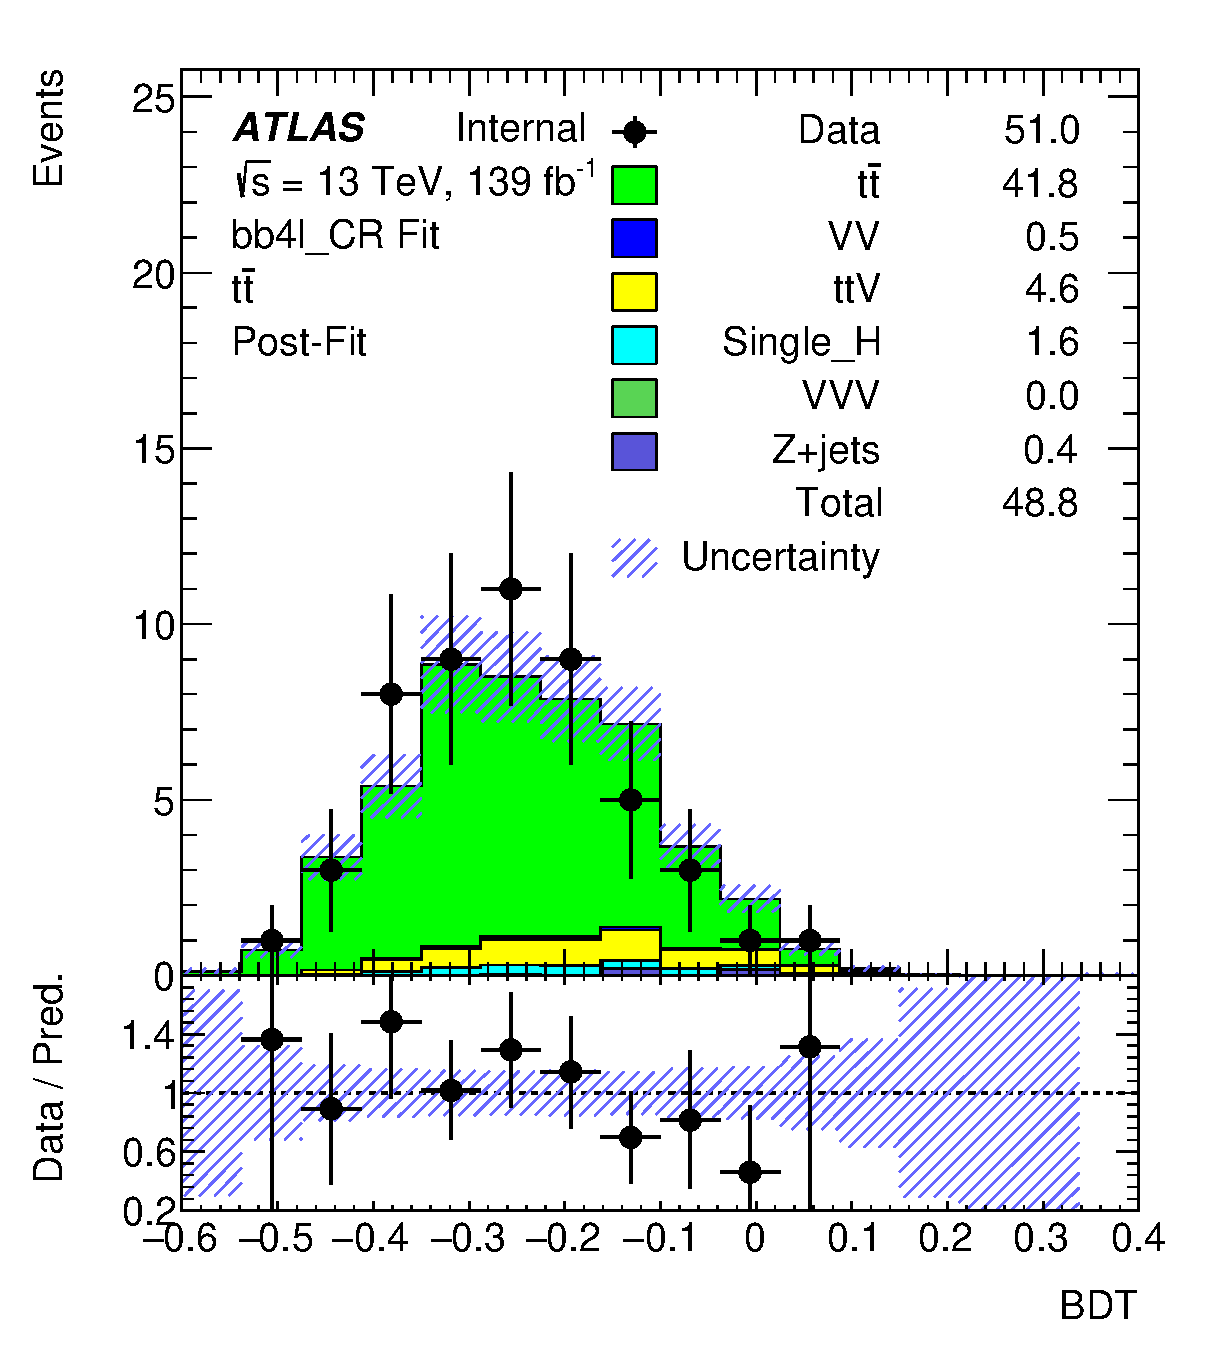
\includegraphics[width=0.4\textwidth]{figures/Plots/tt_CR_postFit.eps}
	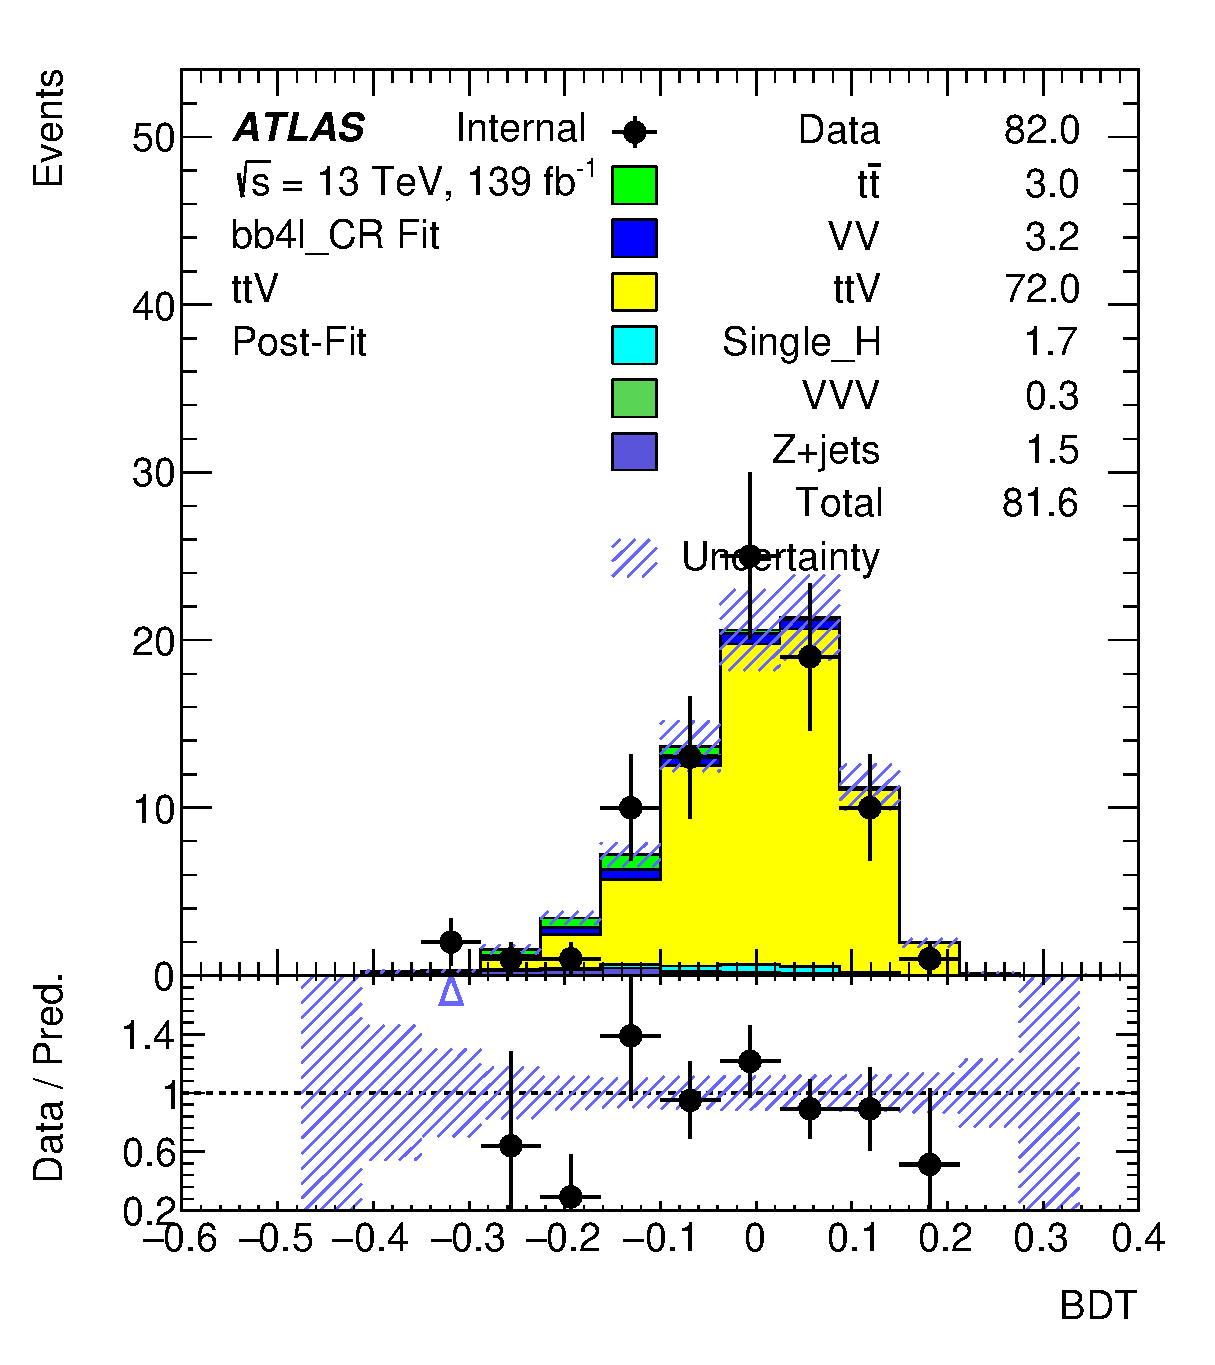
\includegraphics[width=0.4\textwidth]{figures/Plots/ttV_CR_postFit.eps}
	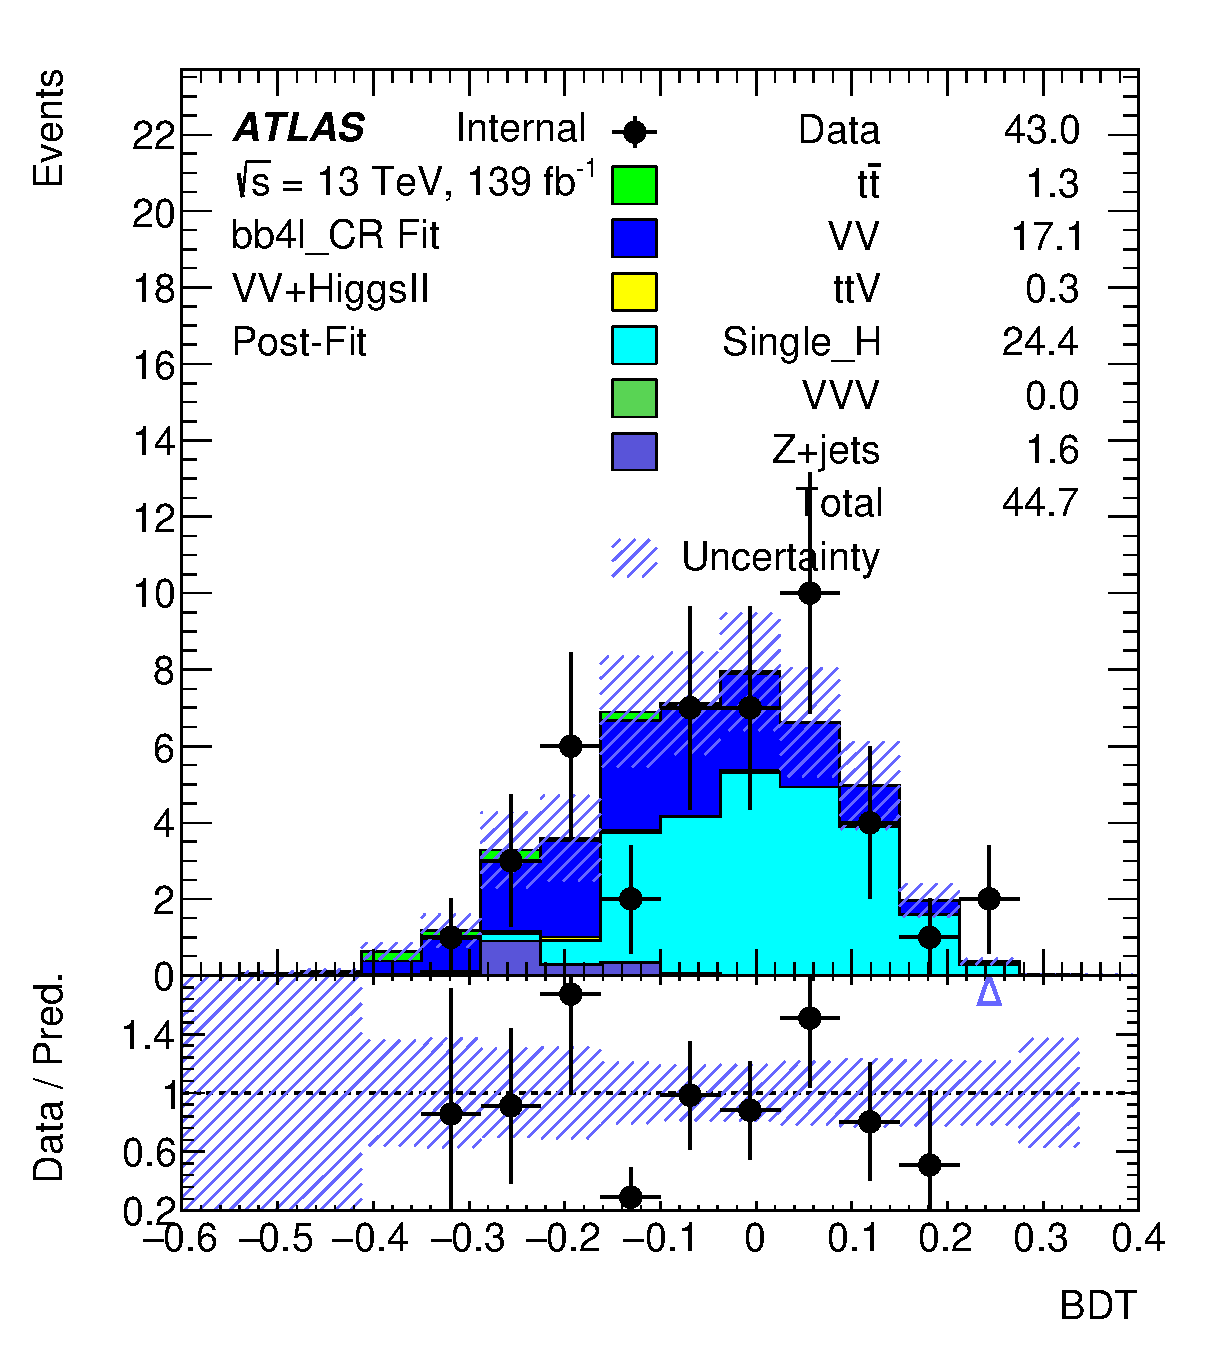
\includegraphics[width=0.4\textwidth]{figures/Plots/VVHiggsII_CR_postFit.eps}
	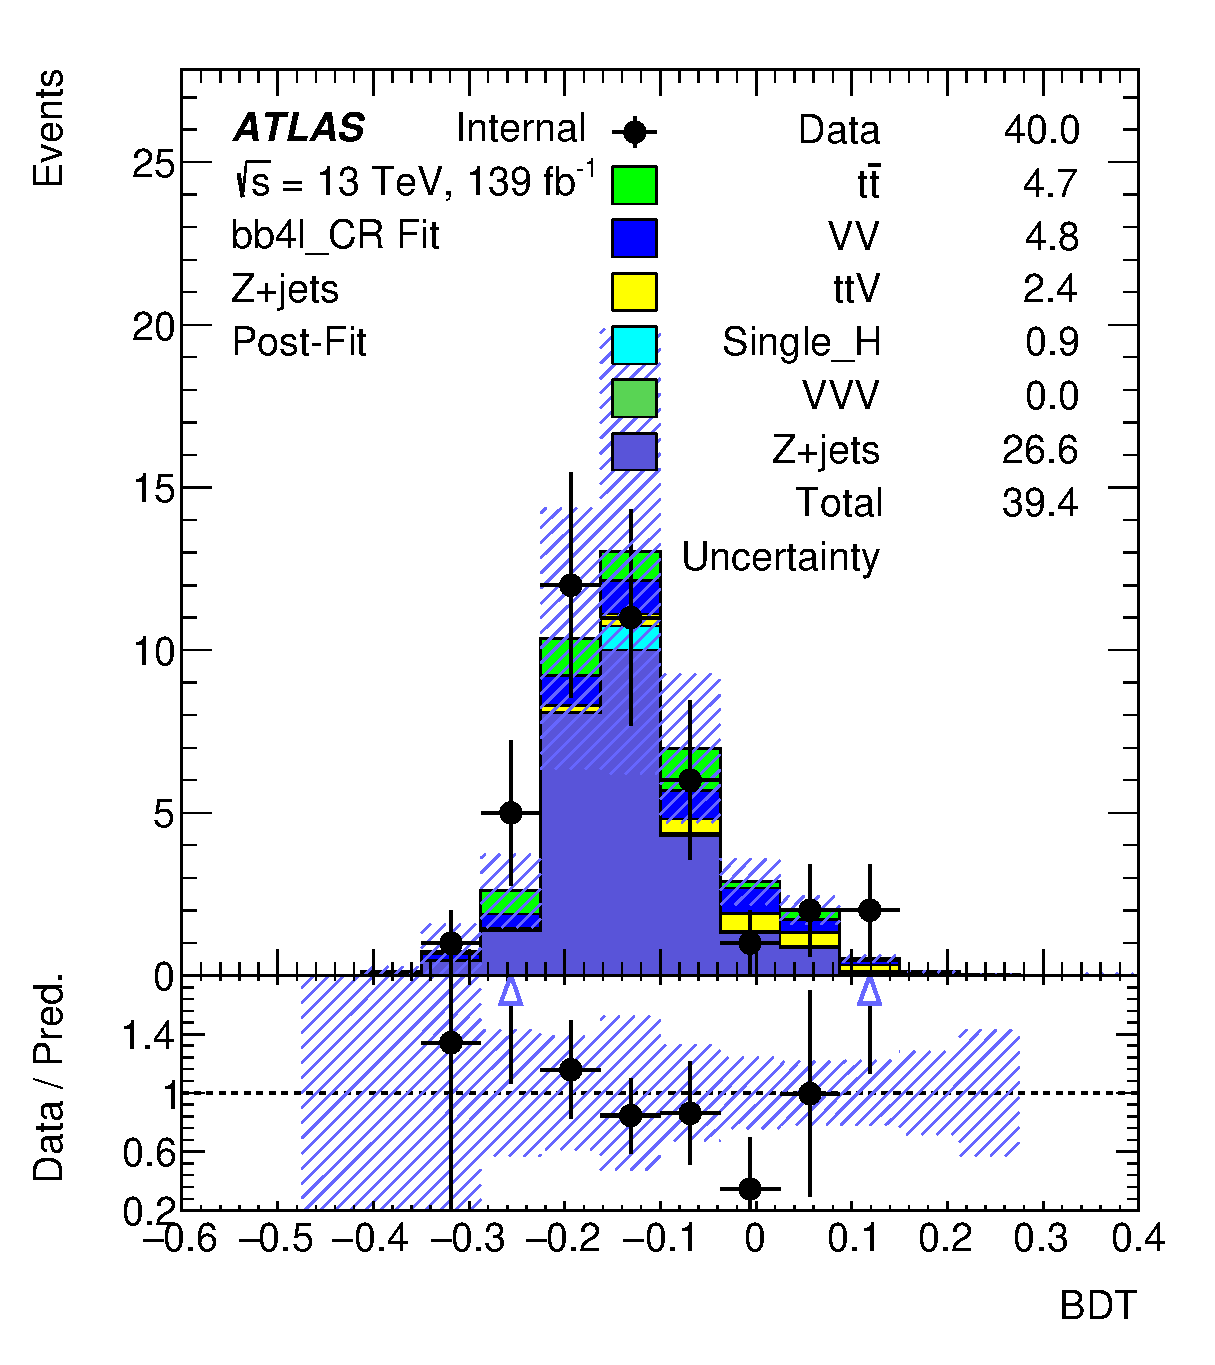
\includegraphics[width=0.4\textwidth]{figures/Plots/Zjets_CR_postFit.eps}
\end{figure}

\begin{figure}[H]
	\caption{Pre-fit and post-fit results in VR, the left one is the pre-fit, the right one is the post-fit.}
	\label{Fig.VR}
	\centering
	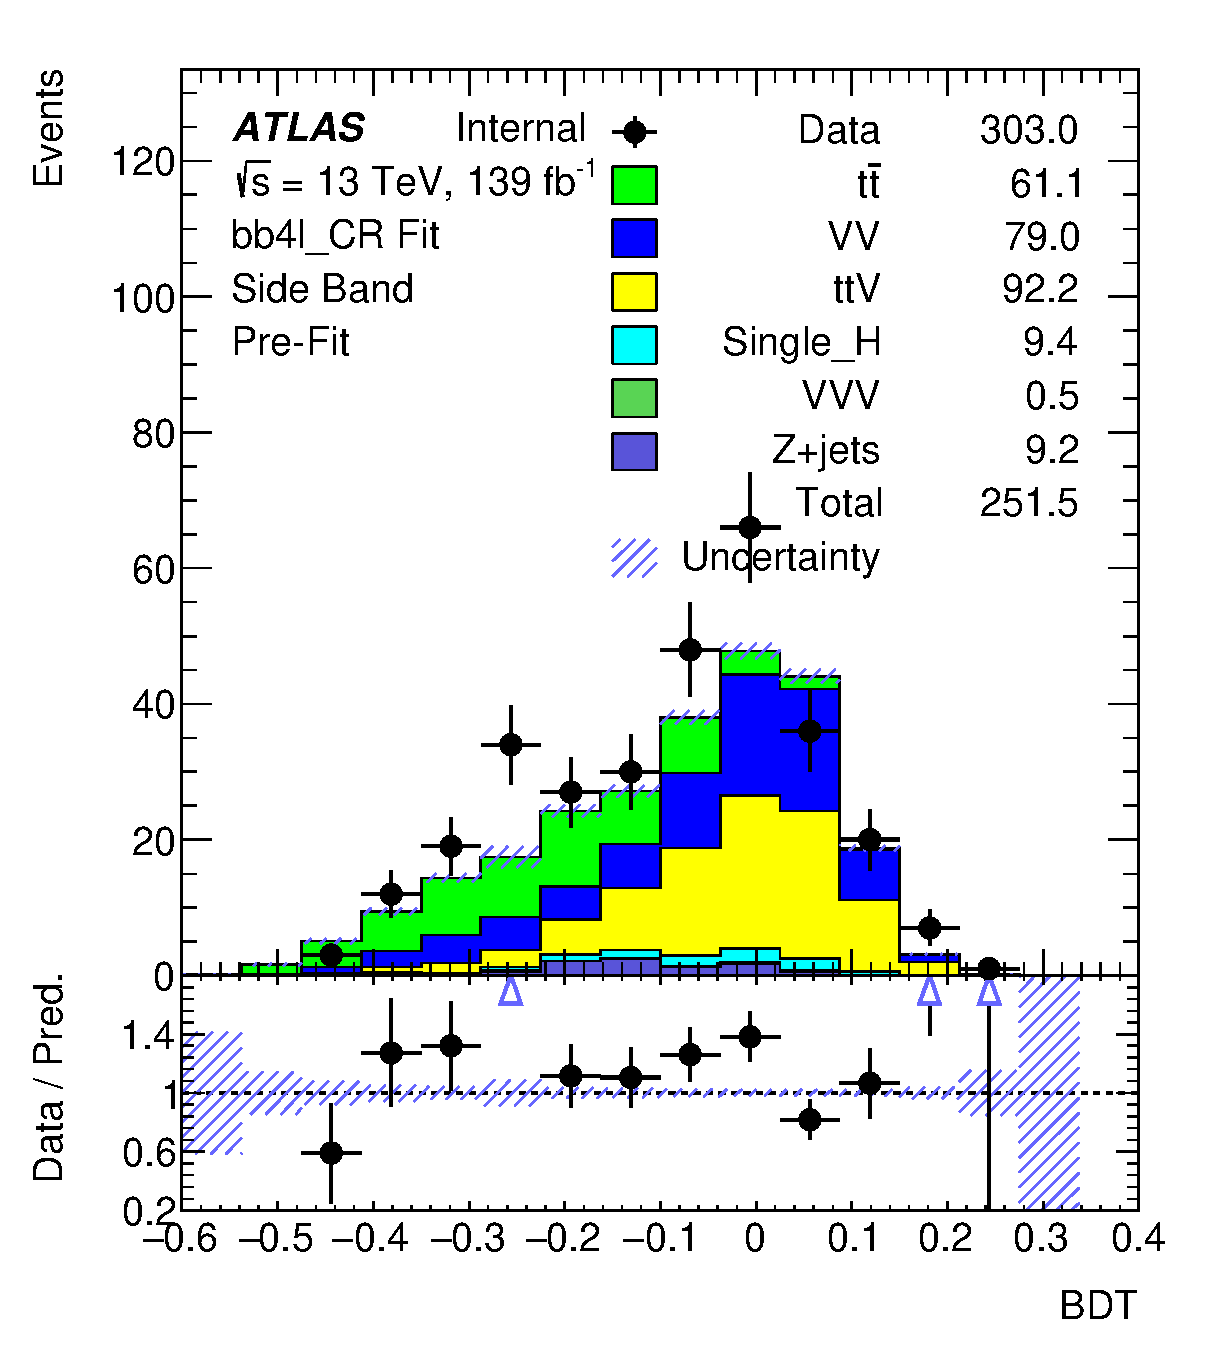
\includegraphics[width=0.4\textwidth]{figures/Plots/VR.eps}
	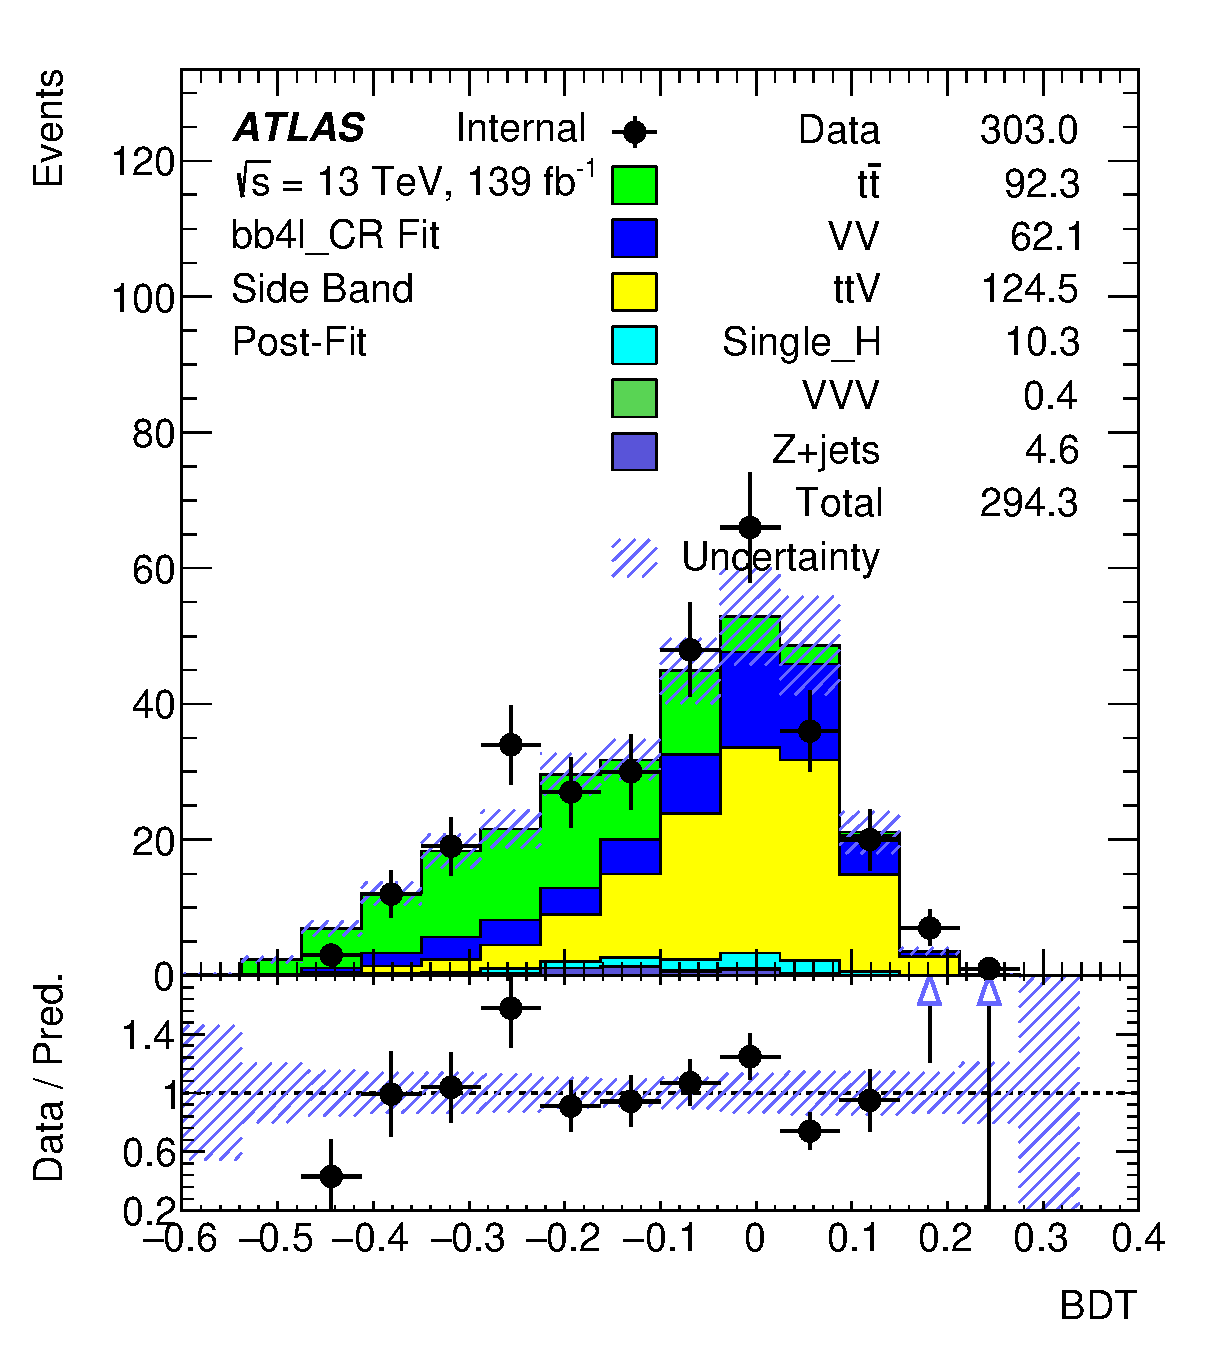
\includegraphics[width=0.4\textwidth]{figures/Plots/VR_postFit.eps}
\end{figure}

\section{Systematic uncertainties}
\label{sec:error}

TBD

\section{Results}
\label{sec:results}

TBD

\section{Conclusions}
\label{sec:conclusion}

TBD
